% ===============================================================================
\section{Structure detection}\label{sec:protocol_structure}
Here we summarize the protocol to follow for generating structure models from stacks of confocal fluorescence images using \wingj. Before starting, we recommend to read carefully the above sections, in particular \sectionref{chap:structure} to understand how structure models are generated in \wingj.\\

The following protocol illustrates the generation of a structure model for the \droso wing pouch from a stack of Wg-Ptc confocal images. A comprehensive flowchart is displayed in \figureref{fig:structure_detection_flowchart}. You can download the \wingjBenchmarkImages to test the structure detection methods implemented in \wingj.

\begin{enumerate}
 \item Set the output directory
 \item Select \textit{\droso wing pouch} from the list of systems supported by \wingj
 \item Import the Wg-Ptc image stack
 \item Give a name to the channel (here ``wg-ptcAB'')
 \item Check that the relation between \px and physical unit (e.g. \mum) is correctly set. If not, edit it in the \emph{Settings}.
 \item Select the structure image channel (optional, by default channel 0)
 \item Select the index of the minimum and maximum z-slices (optional)
 \item Click on \textit{Save} to save image preferences and projections to files
 \item Set an area of interest (AOI, optional)
 \item Click on \textit{Settings} and set the parameter \textit{expectedBoundariesThicknessInPixels}
 \item If the relation ``1 \px = X \textit{unit}'' on the main interface, set the parameters \textit{scale} and \textit{unit} in \textit{Settings}
 \item Click on \textit{Pre-Process}
 \item Automatic detection
    \begin{itemize}
     \item Click on \textit{Run Detection}
    \end{itemize}
 \item Step by step detection
    \begin{itemize}
     \item Click on \textit{Step} to apply one detection module at a time
    \end{itemize}
 \item Manual detection
    \begin{itemize}
     \item Click on \textit{Manual} to display a generic structure to shape
    \end{itemize}
 \item Click on the \textit{tick mark} from the \ij toolbar to validate the structure model
 \item Check that the structure orientation inferred in correct, otherwise edit it
 \item Click on \textit{Dataset} to export the complete structure dataset to the output directory
\end{enumerate}

\textbf{Tip}: Hold your mouse cursor on any elements of the interface to display additional information (tooltips).

\begin{figure}[!h]
\centering
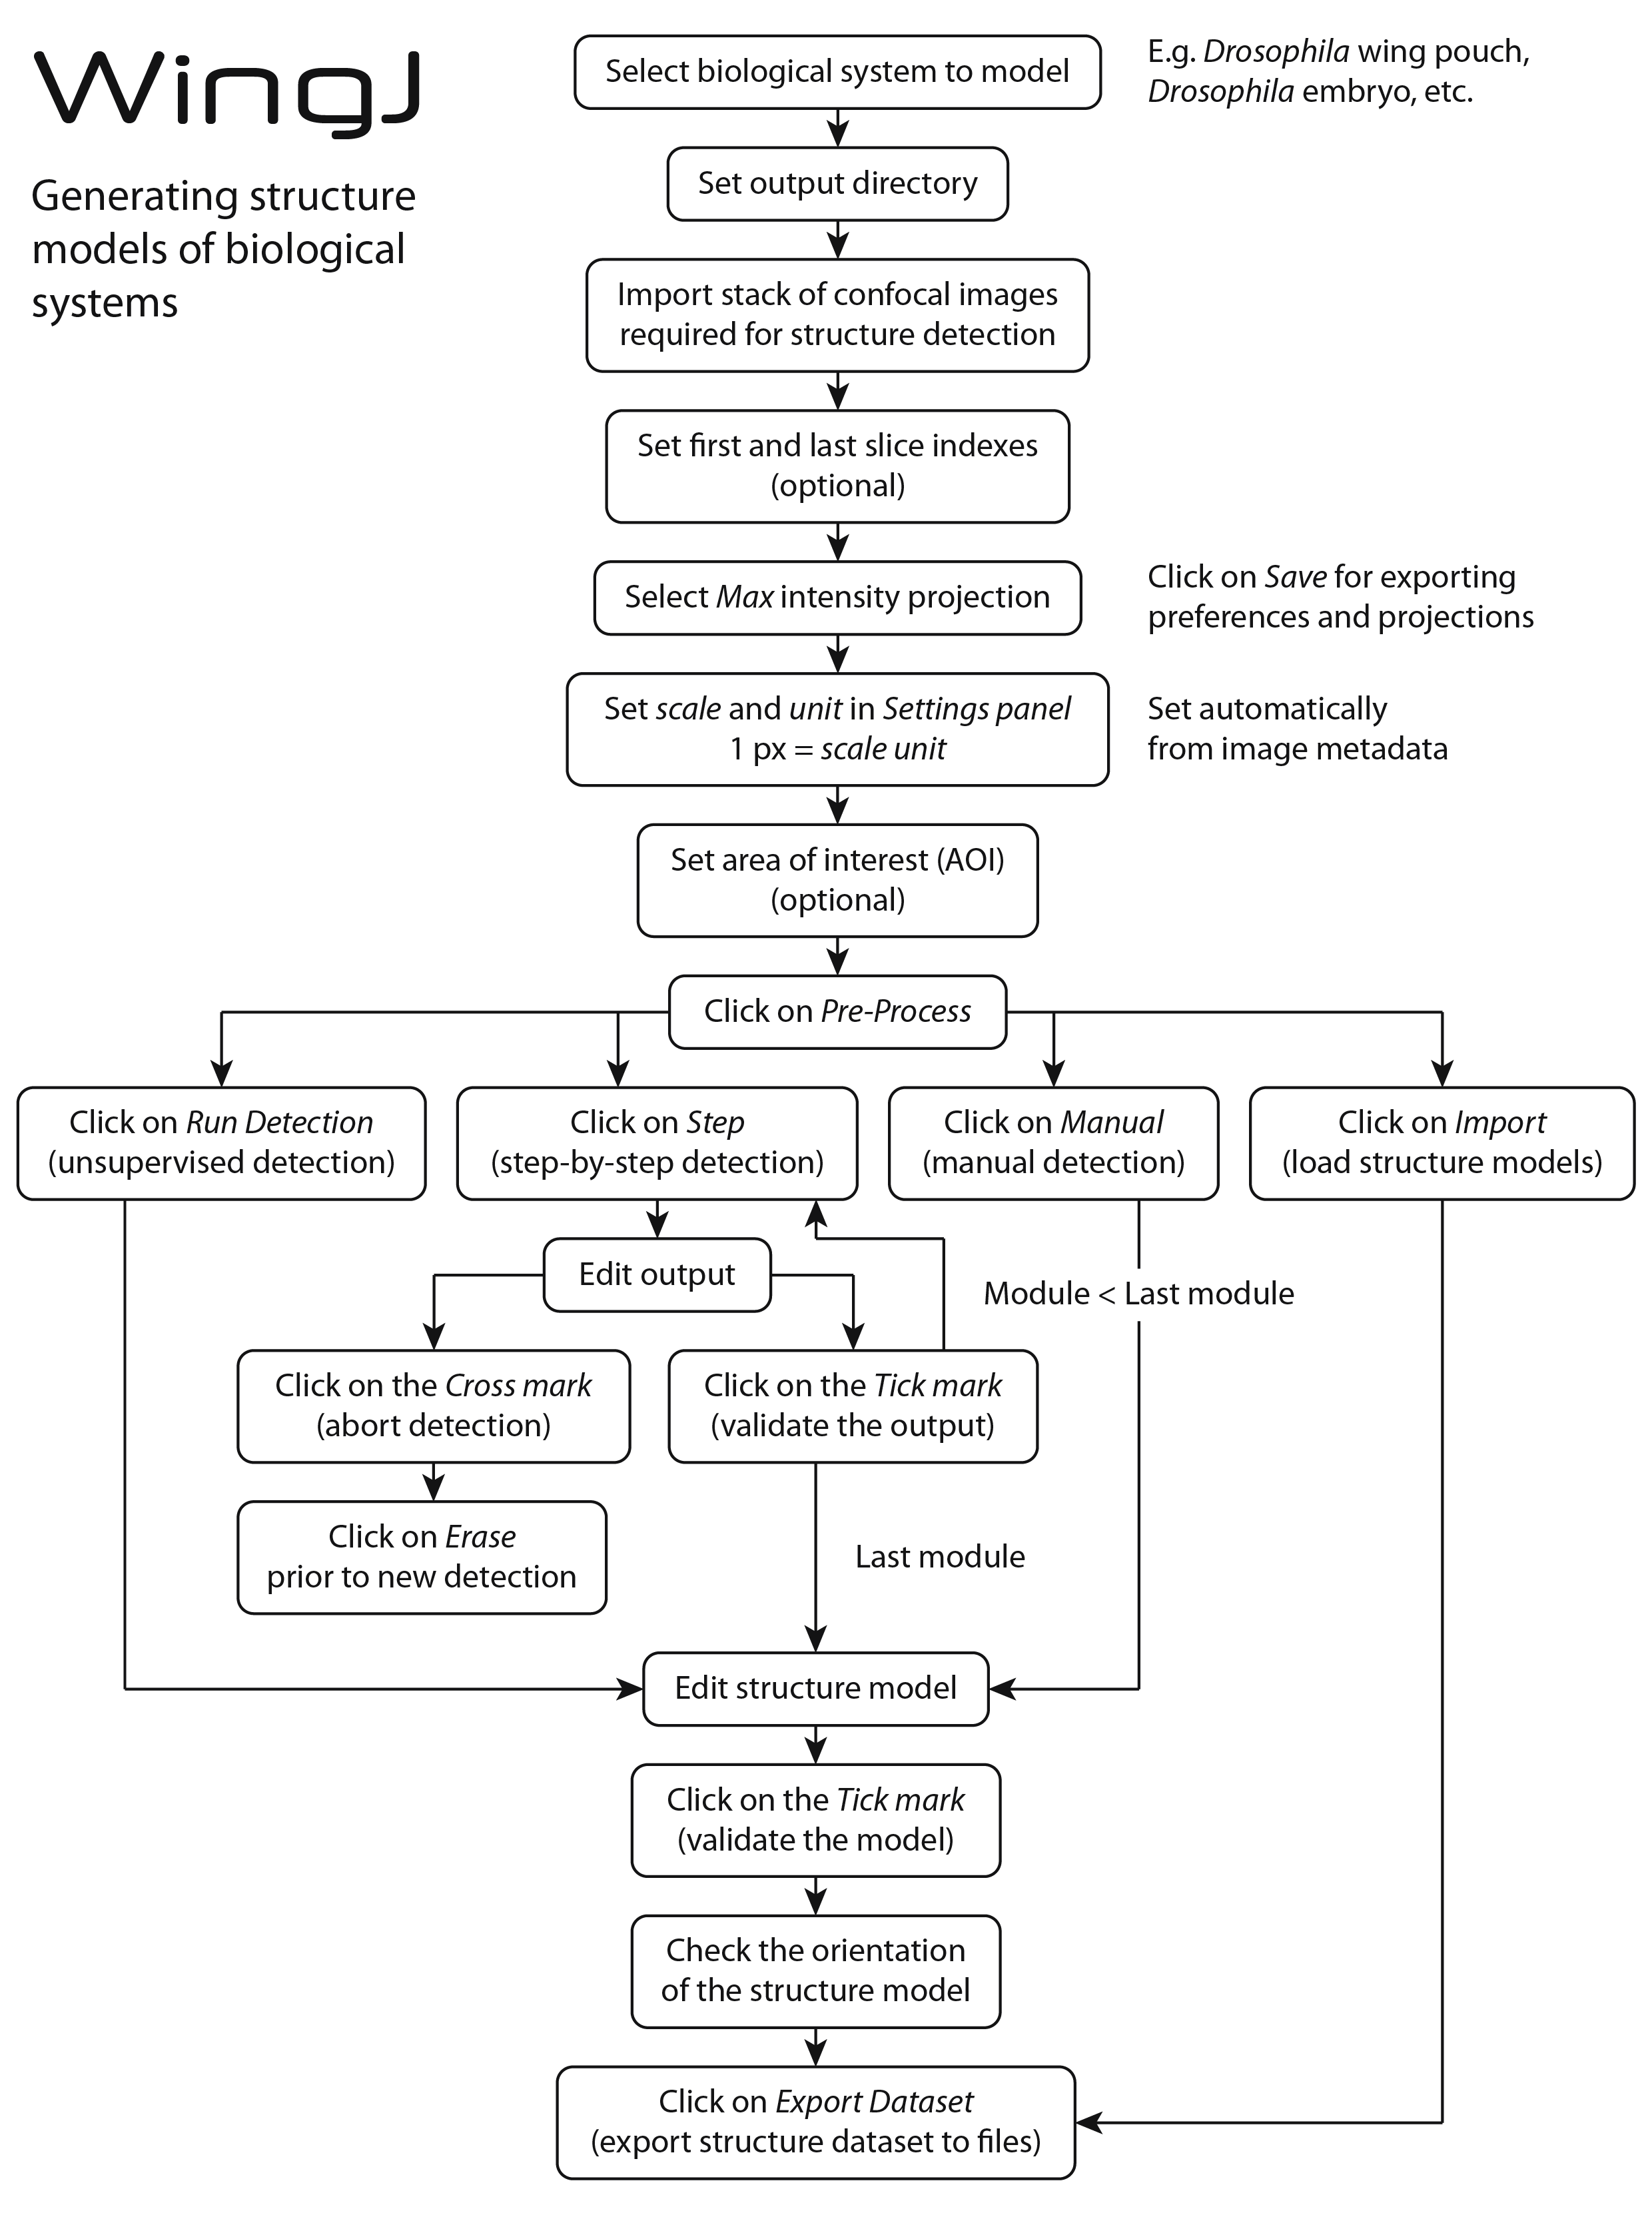
\includegraphics[scale=0.7]{images/structure_detection_flowchart_BW_2.png}
\caption{\textbf{Flowchart for generating a parametric model that accurately describes the morphology or structure of a biological system using \wingj.} This flowchart is also available on the project website along with additional practical information.}
\label{fig:structure_detection_flowchart}
\end{figure}

% ===============================================================================
\section{Expression quantification}
The quantification of gene and protein expression levels from stacks of confocal fluorescence images requires first the identification of a structure model as described in \sectionref{sec:protocol_structure} and \sectionref{chap:structure} for more detailed information. The structure model is then derived to define a non-orthogonal coordinate system within which expression is measured.\\

The following protocol illustrates the quantification of PMad-AB expression from a stack of fluorescence confocal images. A flowchart is displayed in \figureref{fig:expression_detection_flowchart}. You can download the \wingjBenchmarkImages to test the structure detection methods implemented in \wingj.

\begin{itemize}
 \item Import PMad image stack 
 \item Give a name to the channel used (here ``pmadAB'')
 \item Select the index of the minimum and maximum z-slices (optional)
 \item Click on \textit{Mean} to select the mean intensity projection method
 \item Click on \textit{Expression} from the main interface of \wingj
 \item Select the channel to quantify
 \item Check \textit{Normalize} to divide expression level by 255 and thus obtain values in [0,1]
 \item Set \emph{Dataset} to \textit{Individual profiles} to measure expression along a single trajectory inside the structure model
  \begin{itemize}
      \item Set \textit{Boundary} to generate a trajectory parallel to the A/P or D/V compartment boundary
      \item Set \textit{Offset} to translate the trajectory in the anterior/posterior/ventral/dorsal direction
      \item Set \textit{Sigma} to define the width of the measurement domain
      \item Set \textit{Resolution}
      \item Click on \textit{Quantify} to display the expression profile as well as a preview showing where the trajectory along which expression is measured is located inside the structure model
      \item Click on \textit{Export Dataset} to save dataset to files
   \end{itemize}
  \item Set \emph{Dataset} to \textit{Individual maps} to generate individual circular expression maps
      \begin{itemize}
      \item Set \textit{Boundary conserved} to -100\% or 100\% to define whether the expression along the A/P or D/V boundary, respectively, must be conserved in the circular expression map
      \item Set \textit{Stitching smoothing} if \textit{Boundary conserved} is set to a value different from -100\% and 100\%. This parameter can be used to smooth the stitching boundaries.
      \item Set \textit{Resolution} to define the resolution of the circular expression maps in \px
      \item Click on \textit{Quantify} to generate and show the circular expression map
      \item Click on \textit{Export Dataset} to save the circular expression map dataset to files
      \end{itemize}
  \item Set \emph{Dataset} to \textit{Reverse individual maps} to wrap a circular expression map on a structure model
      \begin{itemize}
      \item Select \textit{Use current structure model} to use the structure currently loaded in \wingj as target structure or
      \item Select \textit{Other model} and select a structure model file
      \item Select the \textit{Circular map} to wrap on the selected target structure
      \item Set \textit{Boundary conserved} to A/P or D/V. This choice must be consistent with the selection of the parameter \textit{Boundary conserved} used at the time of generating the circular expression map (see above for \textit{Individual maps} dataset).
      \item Click on \textit{Quantify} to generate and show the circular expression map
      \item Click on \textit{Export Dataset} to save the circular expression map dataset to files
      \end{itemize}
  \item Set \emph{Dataset} to \textit{Mean models} to integrate structure and expression information from multiple experiments in order to generate a robust quantitative description of the selected biological systems.
      \begin{itemize}
	\item Click on \textit{Browse} and select an \textit{experiments repository} (\sectionref{chap:convention})
	\item Set the regular expression for selecting the \wingj structure model files included in the \textit{WingJ} folder of every experiment directory (previously exported to the folder \textit{WingJ} using \wingj)
	\item Set the regular expression for selecting the projection files (previously exported to the folder \textit{WingJ} using \wingj)
% 	      \item Set \textit{Target structure} to select the method to use for generating/selecting the target structure model on which the mean circular expression map is going to be wrapped. If \textit{Synthetic} is selected, the individual structure models available are combined to generate a synthetic structure. If \textit{Area-based} is selected, the individual structure model whose area is the closest to the average area, computed using all models, is selected. If \textit{Manually} is selected, the index of the structure model to use as target structure can be specified (see \textit{Log window} for knowing the index of each experiment).
	\item Click on \textit{Generate} to compute and show the structure and expression aggregated model
	\item Click on \textit{Export Dataset} to compute and export the structure and expression aggregated model
      \end{itemize}
  \item Set \emph{Dataset} to \textit{Composite images} to generate a RGB image from the image stacks opened.
\end{itemize}

\begin{figure}[!h]
\centering
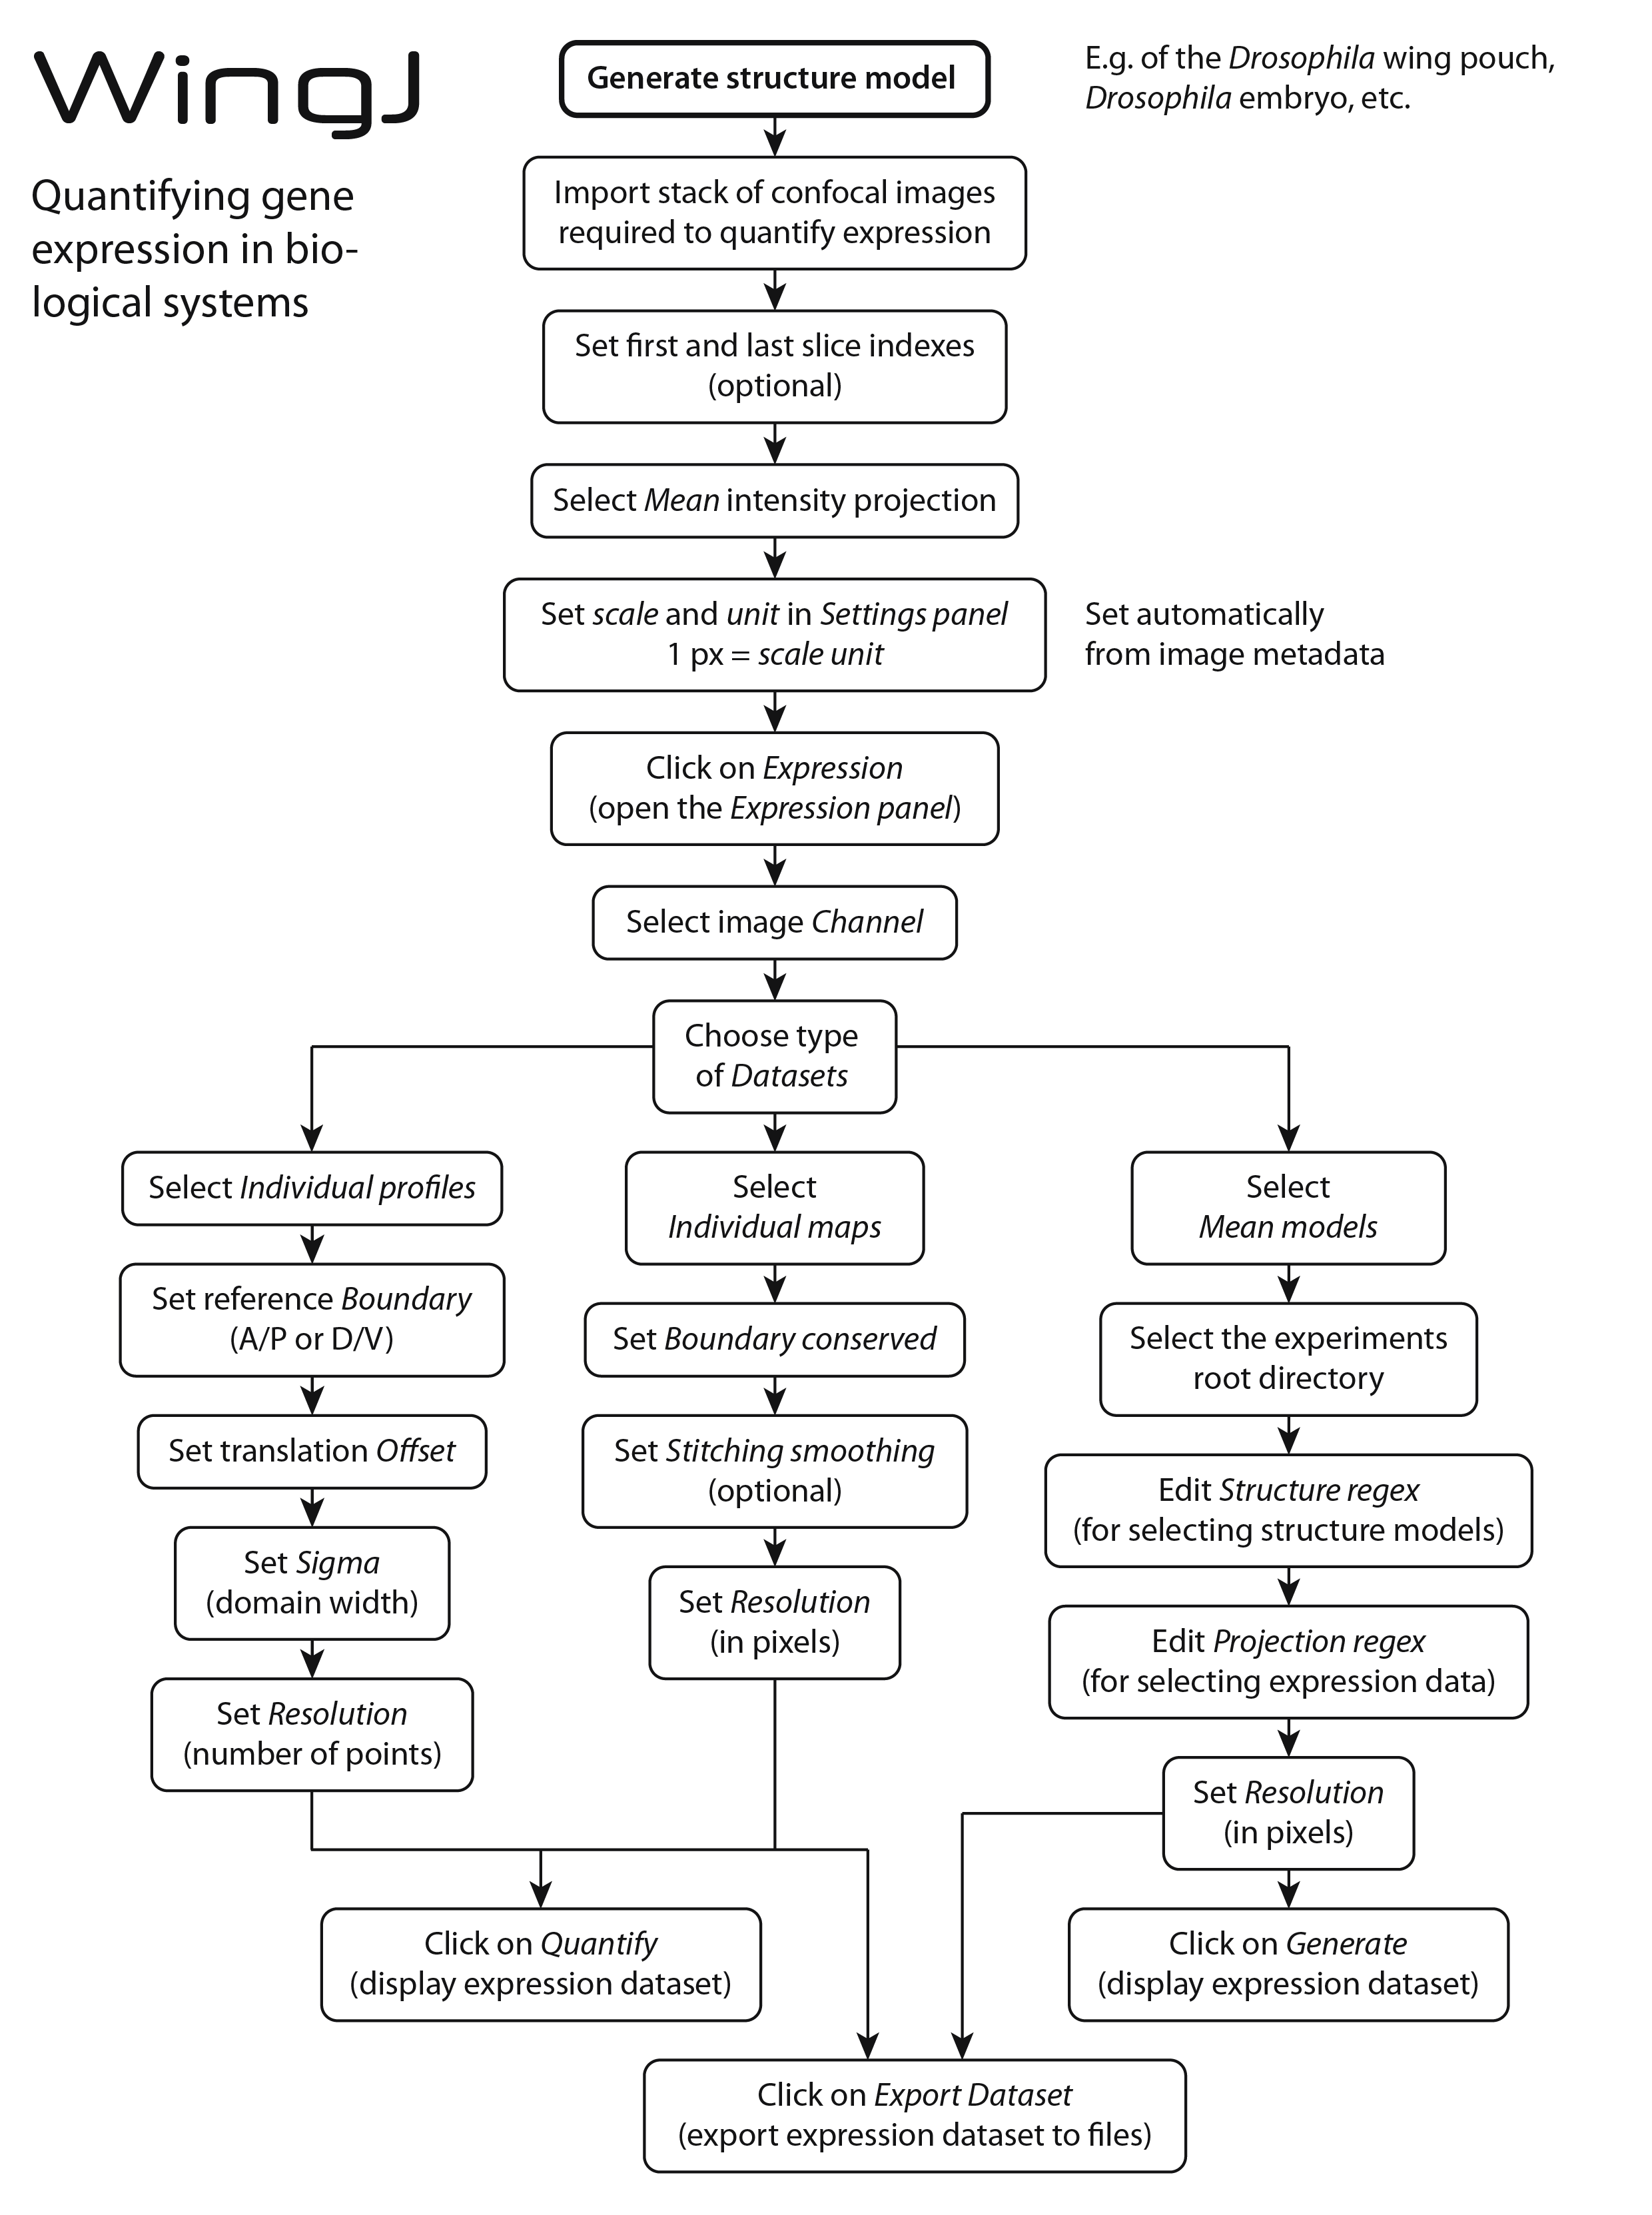
\includegraphics[scale=0.7]{images/expression_flowchart_BW_2.png}
\caption{\textbf{Flowchart for systematic and accurate quantification of gene and protein expression in a biological system using \wingj.} This flowchart is also available on the project website along with additional practical information.}
\label{fig:expression_detection_flowchart}
\end{figure}

% ===============================================================================
\section{\wingjMatlab}
We provide the \wingjMatlab to generate statistics and plots from \wingj datasets. Examples are the generation of statistics from structure measurements (\sectionref{sec:matlab_structure}), the integration of expression profiles (\sectionref{sec:matlab_profiles}), and the 3D detection and segmentation of cell nuclei (\sectionref{sec:matlab_nuclei_detection}).\\

% An exception is the generation of \textit{community expression maps} that can be generated directly from \wingj (Section~\ref{sec:community_expression_maps}).\\

Before starting using the \wingj \matlab toolbox, please have a look at the content of the \matlab file \textit{Settings}. Then, the folder \textit{benchmarks} included in the \wingjMatlab should contain all the data required to run the example scripts. Note that these data may have to be downloaded from separate archives available on the project website (\wingjShortUrl). These data are used by the \matlab scripts \textit{benchmark\_structure.m}, \textit{benchmark\_expression\_profiles.m}, \textit{benchmark\_expression\_maps.m}, and \textit{benchmark\_nuclei} \textit{\_detection.m}. Please refer to the implementation of these scripts for concrete examples on how to use the available tools.